This section describes the purpose, use, and intended user audience for the product "Medtech". Medtech is a system that enables medical professionals to manage patient's medical history, diagnoses, medications, treatment plans, immunization dates, allergies, radiology images, and laboratory and test results. The intended user audience are nurses.

\subsection{Purpose and Use}
Medtech's purpose is to cut down time spent usage. How it should be used in a nurse's normal setting works as follows: Upon logging in with a username and password, the user should see a list of patients. Files to these patients are accessible, and each file includes all medical details and history. To cut down time usage, the user is expected to use the tab search engine if he/she does not know where to navigate.

\subsection{Intended Audience}
Medtech will be publicly available through open source. Since the system scale is small, small clinics would be using this. This product is designed for the sponsor of the project, Dr. Shawn Gieser. Medtech is intended for the nursing component of patient care.

\begin{figure}[h!]
	\centering
   	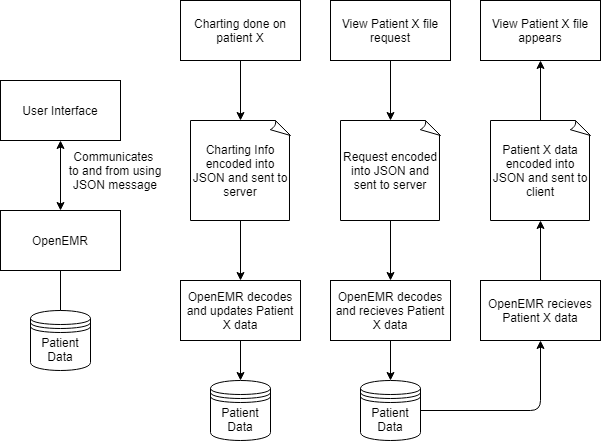
\includegraphics[width=1.00\textwidth]{images/Conceptual Diagram.png}
    \caption{Medtech conceptual drawing}
\end{figure}
